\chapter{Versioning}
\label{chap:versioning}

Versioning determines creation of releases of a product and its management. The product is what provider offers to consumer and its new version is created when a modification is needed. Consumers can use the same product but anyone could use its different version. The version could have been released because of new requirements or due to an improvement of funcionality. 

Any of new versions of the product mustn't influence the execution of consumers code. When the product is customized, a change has to be compatible with all consumers. In case the change is incompatible, it is needed to release a new version. Before a consumer switches the new version an agreement between provider and consumer has to be established. The consumer has to do required changes within usage of the product deriving from the new agreement.

A breaking change is type of change which leads to necessity of modification on consumer side. An example can be a new requirement from one of the consumers, the new version is released and the consumer can immediately switch to use it. Other consumers can follow their schedule and switch to the newest version when it is suitable for them. 

\section{Versioning of services}
\label{sec:verioningservices}
Thanks to versioning, services can be evolved and customized. When a breaking change of service occurs, the new version can be created so that the existing consumers of services are not affected. Release of a new version doesn't harm the previous one, all versions can coexist and be used at the same time. 

\subsection{Version compatibility}
There are two forms of versioning concerning compatibility. \cite{website:service-versioning}
\begin{description}
  \item[Compatible changes] \hfill \\
  Compatible changes are that changes of services which do not harm any consumer. Compatible changes are  for exapmple implemantation bug fixes or change in number of parameters in interface to support an implementation modification.
  \begin{enumerate}
    \item[Backward compatible] \hfill \\ 
  When a new version of a service is deployed the consumer of an earleir version must be capable to interoperate with the new version without any modification of its application. If a service is backward compatible it is compatible with every older version of itself.
  \item[Forward compatible] \hfill \\
  The service version is forward compatible when it is designed in a way it can support future modificatications. The newer version of service can be deployed without influence on its usability by consumers. 
  \end{enumerate}
  
  \item[Incompatible changes] \hfill \\
  Incompatible changes are breaking changes which affects a consumer of services. Exapmle is deletion of an action or changing type or order of the parameters of an action.
  \begin{enumerate} 
    \item[Backward incompatible changes]  \hfill \\
    Backward incompatible changes are that changes which break the consumers using an earlier version of service. It means that the new version is no longer backward compatible and do not interpret the data of its earlier version.
    \item[Forward incompatible changes] \hfill \\
    These changes break the forward compatibility of the service. It means that a future version won't be compatible with existent one, modifications of current version don't preserve compatibility.
  \end{enumerate}
\end{description}


\subsection{Versioning on different levels of a service}
As there are three levels of interpretation \emph{service} a change and followed versioning can occur within each of this levels - business abstraction, service interface, service implementation described previously in \ref{subsec:levels-of-serivce}.

\subsubsection{\textbf{Versioning of business service}}
Sometimes it is needed to change the businsess service. It means the business which is abstracted have to be changed. For exmple because of new reqirements due to legislative a business service needs modifications, if this kind of change affects behaviour, semantic or functionality modification of existing service it is easier to create a new service rather then a version. 

\subsubsection{\textbf{Versioning of service interface}}
As metioned service interface is an entry point for consumers to work with the services. Interface can be versioned as well and its change has impact on the consumer application. Compatible changes of the interface are for expamle addition of an action on the other side non compatible change is removal of an operation. When a new action is added noone is using in ad it is optional if somebody would make use of it. When an action is removed, consumers which have been using it are broken. 

\subsubsection{\textbf{Versioning of service implementation}}
The implementation of the service can be changed do that the new service is backward compatible or backward incompatible. The backward compatible modification in this level is sipmle bug fix, the incompatible change are changes which affect the interface of the service.

Changes of the implementation lead to the versioning the code. Compatible changes can be done without necessity of new version, but they can be versioned after specific numbers of changes, just for proper change management. In case of a breaking change, the code has to be versioned. Incompatible changes requires deprecation, code which has been changed needs to be deprecated to not break the consumer code. Deprecation ensures the backward compatibility od breaking changes.

%popis infrasturkury
Lets have a company which has two streams, one where a developmnet proceed and the other one is a staging stream with stable code. At this point the code is versioned, the version in the company can look like {stream name}{verison number}. Code present in the staging stream is possible to build and produce the dll files. Dll files are deplyed on a server. Consumers are connecting to this server to use services. The process can be seen at the picutre \ref{fig:soa-architecture}
%TODO add dll in glossary, add stable in glossary

\begin{figure}[htp] \centering{
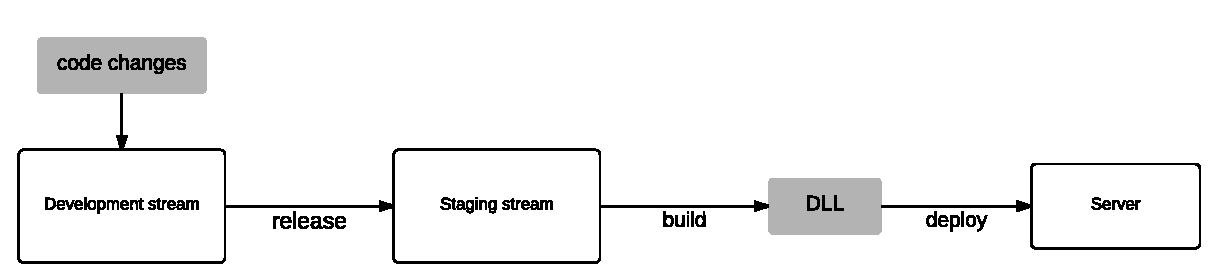
\includegraphics[width=13cm]{img/service-implementation.pdf}}
\caption{Process of deployment of implementation changes}
\label{fig:service-implementation}
\end{figure} 

When a new verison is released into the staging stream code is marked by a version number. The version number is usually composed from four digits {StreamName} X.Y.Z.B where the first change is major change of code and is increased when an important change is done. 
%TODO version number
On the server is just one version of the code. If another version is needed to be availible it has to be deployed on another server. Then customers are using different servers, as shown on the image 

\begin{figure}[htp] \centering{
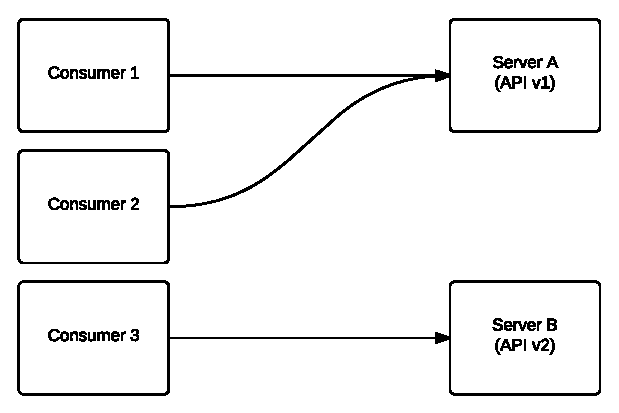
\includegraphics[width=13cm]{img/consumer-server.pdf}}
\caption{}
\label{fig:consumer-server}
\end{figure} 

\subsection{Definition of versioning}

The service layer of application which is developed by the provider is composed of projects containing services, these services has its methods (actions). The design is shown on image \ref{fig:service-layer-design}

\begin{figure}[htp] \centering{
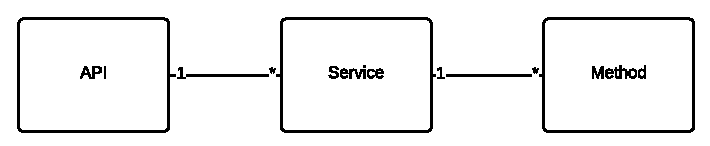
\includegraphics[width=11cm]{img/service-layer-design.pdf}}
\caption{Design of service layer}
\label{fig:service-layer-design}
\end{figure} 

%Each version has its own implementation and is distinguishably addressed.

\bigskip 

Versioning management of services requires the proper definition of following concepts \cite{website:versioning-in-soa}:
%what will be versioned and how, the life-cycle of the versions and the access to the version.
\begin{enumerate}
  \item Units of versioning
  \item Service changes, constituting a new version
  \item Service version life-cycle considerations
  \item Version deployment/access approaches
\end{enumerate}

\subsection{Units of versioning}
It is needed to define what will be versioned, the most frequent are two possibilities:

\begin{description}
  \item[Versioning of project]
  \item[Versioning of service] 
  The whole service is versioned with all its methods. This approach is working well with the object-oriented and the component-base development. It's not appropriate with coarse-grained services \ref{sec:granularity}.(3)
  \item[Versioning of service method] 
  In most cases the change arises just in a method or some methods of the service. It is not neccessary to version the whole service, but there is an option to verison just these operations.
  The benefits of this approach are less code which is deployed because just a changed methods are redeployed in a new version. All services are immutable, their name and classification remain unchanged when there is a method added. The changes concern just a consumers which use the method, instead of consumers of the service containing changed method. 
  When the versioning of method is used it is needed to deploy each method with its own endpoint address, the advantage is that the \gls{sla} is provided fot the method so that it is not changed the SLA of the same service.
  Moreover the addressing schema becomes more complex, the consumer has to specify not just the service but also the method and version of method which wants to use.
In spite of the more elaborate routing this possibility of versioning offers more flexibility. It adapts the services versioning to versioning practices of commonly used programming languages. 
Other benefit of this approach is deprecation, an old method which has new vesion can be signed as deprecated. The method can become deprecated when a better alternative is implemented but there are still consumers which use the old one. This method can remain in service until all consumers switch to the newest method.
\end{description}

\subsection{Version definition}
It is necessary to analyze the services/methods from the point of view of changes, their impact on the consumer. Analysis of possible changes deals with influence of change on the consumers execution and consequntly defines the changes which will break it. When the change of the service or method is breaking it leads to the creation of new version.

The components of the service are interface and message, both of them could be changed and cause the release of new version.

\subsubsection{Interface changes}
A change of interface has significant impact on the consumer, it requires many modification of customers implementation or even completely new service. The deprecation of a method is equivalent to its removal and should occur rarely.
When following semantic messages model, the interface is never changed. Advatage of this approach has source in the fact that all changes can be done just within the methods of service. When the methods are units of versioning they are deployed individually and new methods can be added without any impact on existing consumer. When the method is going to be removed, it is first deprecated, so that is still kept around the service and could be used until all consumers stop to use it. The changes are contained in messages and are not shown whitin the interface.
Than as seen it is better to desing the versioning defintion in order to not include the interface changes.

\subsubsection{Message changes}
When using the semantic message model the changes of service interface do not change the interfac itelf but are contained in message. The message is created by a schema which describes its content. Chenges in schema can provide different cases of compatibility wit actial implementation and can be divided in three categories:

\begin{enumerate}
  \item[Revisions]
  Revisions are changes without semantic content, for exapmle formatting, comments, etc. They do not affect the functionality of the service and service consumers.
  
  \item[Minor changes]
  Minor changes are backward-compatible changes of document schema, that means the changes do not impact consumers, the new version continue to support the consumers working with the old version. Examples can be new optional element to existing type, a change of optionality of a local element from required ot optional, adding global type or global element, etc.
  
  \item[Major changes]
  Major changes are non-backward compatible changes, after a major change the new document schema is no longer compatible with the old one. These chagnes are breaking the usage of the service by the consumer. They are imposed to the new version and consumers need to adjust its program to switch to this version. Breaking changes can be performed by adding or removing an enumeration, removing or renaming a global type or element, changing the optionality of an element from optional to required.
\end{enumerate} 

\subsubsection{Implementation changes}
Interface defines the serivce and make the access point from the consumer point of view. The underlying implementation is encapsulated and not visible for outer world. Depite this the implementation cannot be replaced without affectiong the whole service. A provider of service has the contract including SLA \gls{sla} with a service consumer. The contract has to be followed because it is valid document on which the consumer relies. 
Every change which has to be done in the implementation of the service needs to be validated against the contract. When the implementation which is going to be replaced is the breaking change from the point of view of the consumer the agreement with the change of contract is needed and consequently the new version has to be released.

\subsection{Service version life-cycle}
Service life-cycle defines the time period in which a version should be maintained. When the time is short, customers have not enough time for their upgrades required in order to swich on new verion.l On the other hand when the period is too long, too many versions of service have to be maintained. The suitable time span is a result of consideration of individual organization with respect to their capability to deal with changes.

Product verions should be always compatible with consumers usage. When a new version of the service method is released, it is needed to have the old one present in the implementation if any of the consumers operate with it. When the service method is going to be replaced by new one, it has to be hold so that do not impact any consumer. It can be signed as deprecated, which do not influence its usage from the point of view of the consumer, but it means that provider waits that all consumers switch to the new implemenation. When the deprecated method stops to be used, it can be safely removed. 

This lifecycle is posible only when the service method versioning approach is implemented, in case of whole service versioning, when the service is given into state deprecated, it is equvalent to its remove, it is needed the new agreement between the provider and consumer so that consumer have to implement changes to use the new service or just  keep useng the older version. The whole serivce versioning provides less flexibility.

\subsection{Version access}
It is needed to define how different consumers of services are accessing its verion of the service. There are several approachs everyone has its pros and cons. The access posibilities are described in separate chapter \ref{chap:versionaccess}.

\section{Versioning service implementation}
Besides versioning the service interface, it is possible to consider an implementation. The underlying implementation can changed without affectiong the interface itself. 
